In this section, basic approaches how to focus a laser beam in experiments are discussed. Before providing a brief overview of currently used methods, it is necessary to introduce several most fundamental parameters that describe any optical system. First, one defines a numerical aperture of an optical system $ N\!A $, which is a dimensionless number characterizing the range of angles over which the system can accept or emit light. Second characteristic of any optical system is a focal length $ f $ describing a distance between the center of the aperture and the point in space over which collimated light rays are brought to a focus. Finally, one defines a f-number $ f/\# $ as a ratio of the focal length $ f $ to the size of the aperture $ D $. The f-number is dimensionless and stands for a quantitative measure of a speed of the optical system.

In experiments, focusing of laser beams is usually achieved by means of an optical system, such as a lens or a curved mirror. However, when dealing with a short pulses, lenses are not preferred because they may affect the beam by frequency-dependent effects, such as chromatic aberration and other nonlinear optical distortions. On the other hand, reflective optics are generally able to produce a diffraction limited image without chromatic effects.

An off-axis parabolic mirror is a frequently used tool to focus an incoming collimated beam. It is made by cutting out a small section from a full parabolic mirror and thus it allows to deviate the beam path off the optical axis. Therefore, the focal point is at more accessible location and the target is not blocking the incoming collimated laser beam as in the case of a complete parabolic mirror. Obviously, the off-axis parabolic mirror is able to work reversibly, so it can take the light coming from a point source and produce a collimated beam. These physical properties make the off-axis parabolic mirror a valuable tool for many different optical purposes.

However, as soon as the laser intensity exceeds $ 10^{13} \ \mathrm{W/cm}^{2} $, the surface of any material becomes strongly ionized. Therefore, in order to keep the energy density on the optical components below the damage threshold, the beam diameter has to be increased. This approach inherently imposes limits upon the geometrical characteristics of the focused beam such as the size of the focus. The focal spot can be alternatively decreased by implementing a small f-number focusing optic. However, since their focal length is inevitably very short and therefore they must be placed in close proximity to the interaction region, additional care has to be taken to protect the optical components because they can be easily damaged from debris induced by the exploded target flow. Note that such optics are typically very expensive.

\floatsetup[figure]{style=plain, subcapbesideposition=top}
\begin{figure}[h!]
	\centering
	\sidesubfloat[]{{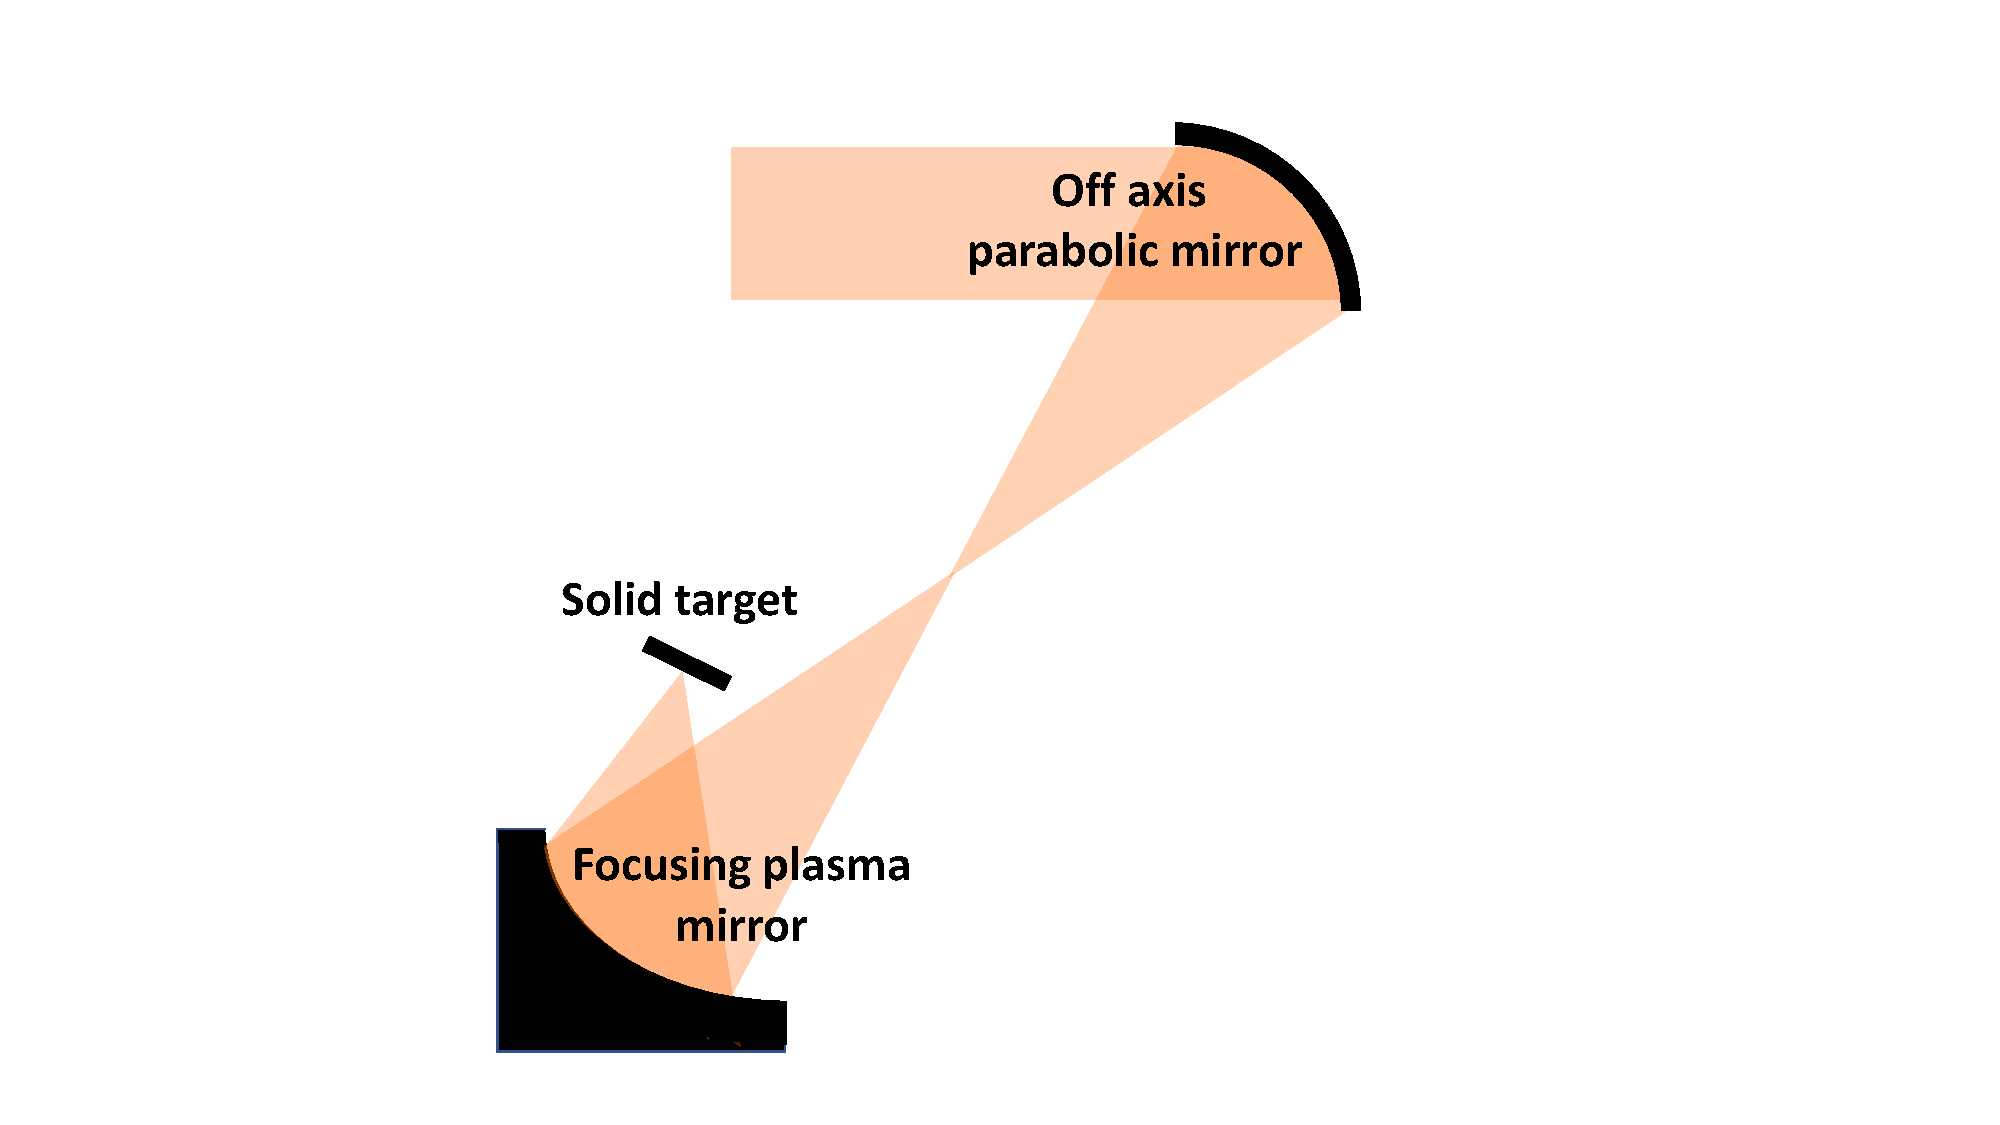
\includegraphics[width=0.35\linewidth]{./img/exp/diagram.pdf}}}
	\hspace{5mm}
	\sidesubfloat[]{{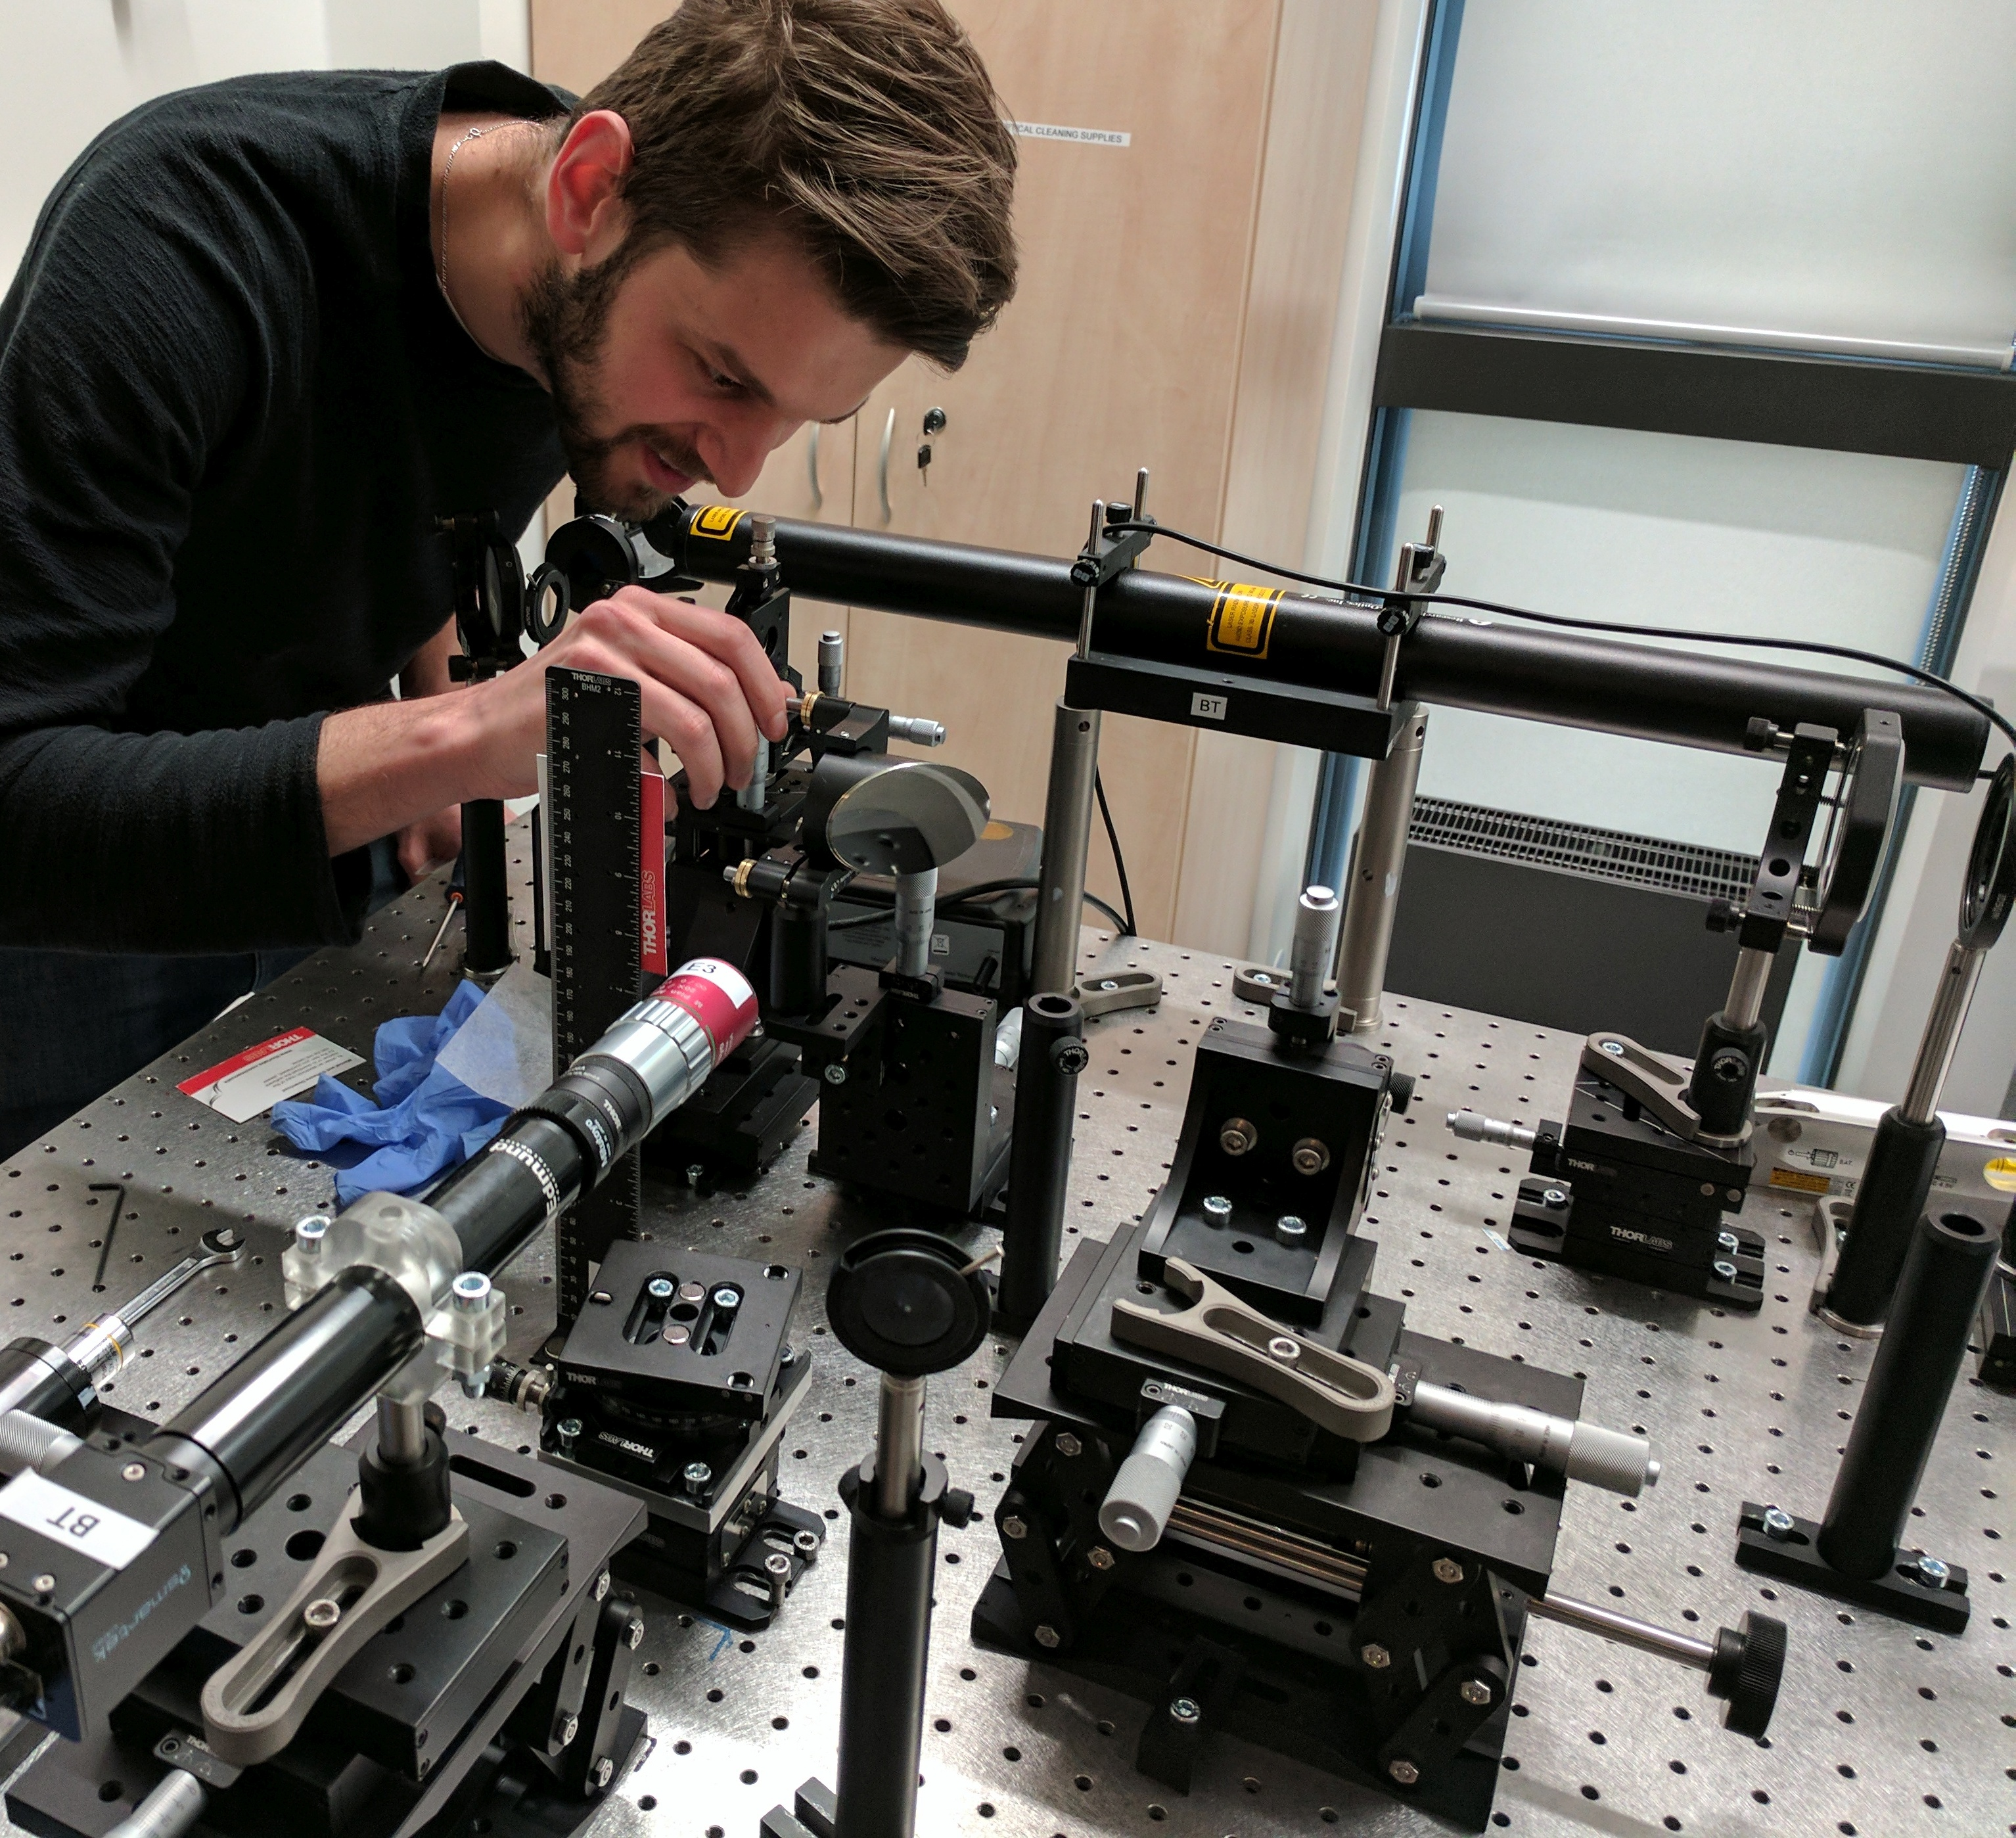
\includegraphics[width=0.4\linewidth]{./img/exp/photo2.jpg}}}
	\caption{\textbf{(a)} Schematic diagram showing the experimental set-up for tight-focusing. The incoming laser beam is focused by a conventional off-axis parabolic mirror to the first focal point of the ellipsoidal plasma mirror, beyond the light diverges and is reflected from the dense plasma created on the surface of plasma mirror. The beam is then imaged to the second focal spot where the target should be placed. \textbf{(b)} Photo taken at Extreme Light Infrastructure (ELI) laser facility capturing a very long and frustrating procedure of aligning an off-axis parabolic mirror.}
	\label{fig:9}
\end{figure}

In the case of tight-focusing, the conventional solid state optics seems to be inappropriate. Nevertheless, many of the drawbacks mentioned above might be overcome by using a plasma-based focusing optics. As already mentioned in the chapter 2, when the laser pulse with intensity higher than $ 10^{16} \ \mathrm{W/cm}^{2} $ hits a solid target, a thin dense plasma layer is immediately formed on its surface. Under certain conditions, the plasma becomes dense enough and the reflectivity of otherwise transparent target strongly increases. The incident laser light is reflected at the critical plasma density, thus the dense plasma acts as a mirror. These optical components are known as plasma mirrors.

Plasma mirrors are able to operate under much higher energy density than the conventional solid state optics, therefore the optics aperture diameter can be more than one order of magnitude smaller. Consequently, plasma mirrors can be mass-produced at much lower cost, which is crucial since they are single-use and thus have to be replaced after each shot. In addition, the concerns about damage from target debris are naturally eliminated.

To induce focusing, the surface of plasma mirror has to be curved similarly as in conventional optics. However, since the distance between the mirror and the interaction region can be significantly reduced, the corresponding f-number can be extremely small enabling to focus an incident laser beam to a spot size smaller than the center laser wavelength. In addition, plasma mirrors are attractive also due to their ability to improve the temporal and spatial contrast ratio of the laser pulse, which is crucial for many applications of the laser-matter interaction.

The diagram in Fig. \ref{fig:9} - a schematically shows an experimental configuration for tight-focusing. A conventional off-axis parabolic mirror is aligned in such a way that the focus coincides with the first focal point of the ellipsoidal focusing plasma mirror. The ellipsoidal shape of the mirror is chosen because it enables point-to-point imaging, possesses no spherical aberration and allows relatively simple alignment procedure. The light reflected from the plasma mirror is then imaged to the second focal spot. The Fig. \ref{fig:9} - b shows the alignment procedure of the off-axis parabolic mirror in practice.

Alternative to plasma mirrors could be a plasma lens. This concept is based on creating a short plasma channel which is able to guide an intense laser pulse. Similarly as for the plasma mirrors, plasma lens would tolerate laser intensities above the damage threshold for conventional solid state optics and allow to manipulate with the laser beam in close proximity to the interaction region. The focal length of the plasma lens is expected to be independent of the laser intensity as long as the interaction regime is non-relativistic. The plasma lens may, in principle, be tuned by controlling the plasma density. Consequently, it would be possible to change the position of the focal point without physically moving any optical element [source].

The last approach reviewed in this work,

%Lens, off-axis parabola mirror - conventional solid state optic
%ellipsoid plasma mirrors, plasma lens
%wedge targets